%!tex root=./thesis.tex

\appendix

\chapter*{Appendix}
\addcontentsline{toc}{chapter}{Appendix}
\markboth{Appendix}{}

\renewcommand{\thefigure}{\Alph{section}.\arabic{figure}}
\renewcommand{\thetable}{\Alph{section}.\arabic{table}}
\renewcommand{\theequation}{\Alph{section}.\arabic{equation}}
\numberwithin{figure}{section}
\numberwithin{table}{section}
\numberwithin{equation}{section}


  \section{Sankey diagrams}
  \label{sec:rlfs-sankey}

    This section presents Sankey diagrams showing the filtering of components and sources from the full FIRST sample in \autoref{cha:rlfs}, and was originally an appendix to \citet{alger21rlfs}. A Sankey diagram shows the order and number of objects removed from a sample. \autoref{fig:sankey-components} shows the filtering of components and \autoref{fig:sankey-sources} shows the filtering of sources. The component filters are `Bad FIRST' for components on the edge of FIRST with incomplete images, `Sidelobe' for components with high sidelobe probability, `Low score' for components with only low-scoring candidate hosts, `Faint' for components with less than 10 signal-to-noise according to the FIRST catalogue, and `Compact' for components that do not have extended radio emission according to \autoref{eq:rgz-criterion}. Sources were removed after each component filter if they no longer contained any components.

    \begin{figure}
        \centering
        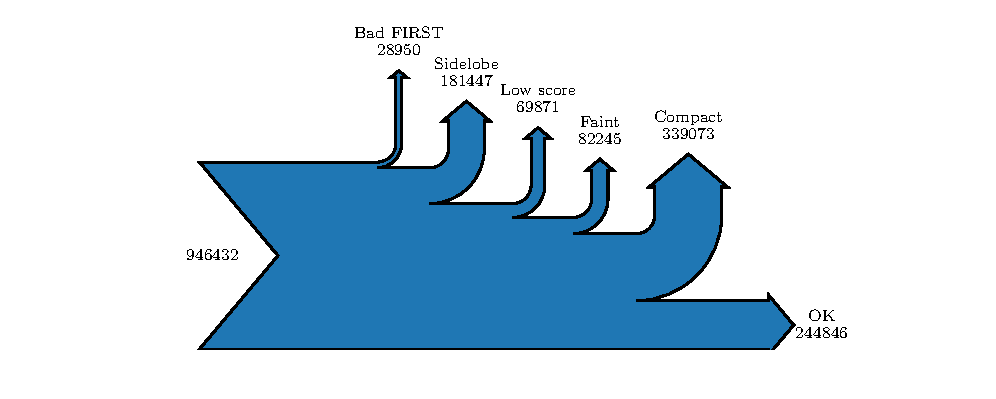
\includegraphics{rlf-images/sankey_components.pdf}
        \caption{\label{fig:sankey-components} Number of components removed from FIRST by each filter.}
    \end{figure}

    \begin{figure}
        \centering
        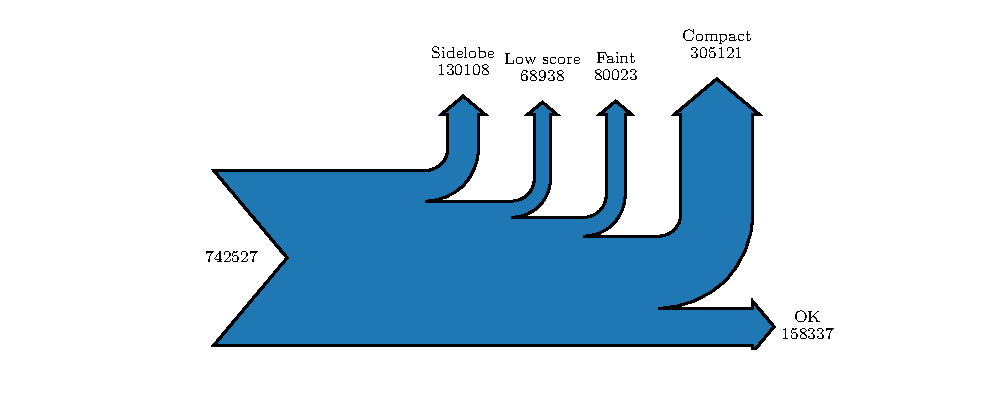
\includegraphics{rlf-images/sankey_sources.pdf}
        \caption{\label{fig:sankey-sources} Number of sources removed by each filter.}
    \end{figure}

\section{Radio luminosity function}
\label{sec:rlfs-rlf-desc}

  We computed the radio luminosity function following the $1/V_{\max}$ method
  \citep{schmidt1968vmax}. This appendix explains our implementation in \autoref{cha:rlfs} and was originally an appendix to \citet{alger21rlfs}. We performed the
  following steps:
  \begin{enumerate}
    \item Remove all radio sources that do not fit the selection criteria.
      This applies for both radio and infrared properties, so we choose a minimum radio flux density $f_{\min}$ and a maximum infrared magnitude
      $m_{\max}$, as well as redshift limits $z_{\mathrm{lower}}$ and $z_{\mathrm{upper}}$.
    \item For each source, compute the maximum redshift that the source could
      have been observed within the selection criteria. We find this redshift
      by first numerically solving \autoref{eq:luminosity} for $z$ with $L$ as
      the luminosity of each radio source and $f = f_{\min}$ to obtain the
      maximum redshift $z_\text{radio}$ at which the source could be observed
      in radio. We find the maximum redshift $z_{\text{ir}}$ that the host
      galaxy could be observed within the selection criteria by numerically
      solving \autoref{eq:ir-limits} for $z$, where $d(z)$ is the luminosity
      distance at a redshift $z$, $d$ is the luminosity distance of the host
      galaxy, and $m$ is the apparent magnitude of the host galaxy.
      \begin{equation}
        \label{eq:ir-limits}
        5 \log_{10}\left(\frac{d(z)}{d}\right) + m = m_{\max}
      \end{equation}
      The maximum redshift that the source could have been observed within the
      selection criteria is then $z_{\mathrm{max}} = \min(z_{\mathrm{ir}}, z_{\mathrm{radio}}, z_{\mathrm{upper}})$.
    \item For each source, compute the comoving volume $V_{\mathrm{max}}$ at
      redshift $z_{\mathrm{max}}$.
    \item The count for each luminosity bin is the sum over $1 / V_{\max}$ for
      each source in the bin. We divided these counts by the estimated completeness (\autoref{sec:rlfs-completeness}) to account for redshift incompleteness.
      We account for the fact FIRST does not cover the
      whole sky by multiplying by the total area of the sky divided by the area
      of our selection.
  \end{enumerate}

  After computing the luminosity function, we estimate the uncertainty in each bin using Poisson statistics, $\sqrt{N}$ for a bin count $N$.

  \section{Redshift completeness estimate}
  \label{sec:rlfs-completeness}

    \autoref{fig:completeness-wise} shows the estimated completeness of our RLF sample in \autoref{cha:rlfs} as a function of $W1$ and $W1-W2$. We followed the same method as \citet{pracy16rlf} for this estimation, averaging completeness over circles centred on each source. Each source is associated with a circle of radius equal to the distance to its 50th nearest neighbour in the $W1$ and $W1-W2$ plane. This appendix was originally part of \citet{alger21rlfs}.

    \begin{figure}
        \centering
        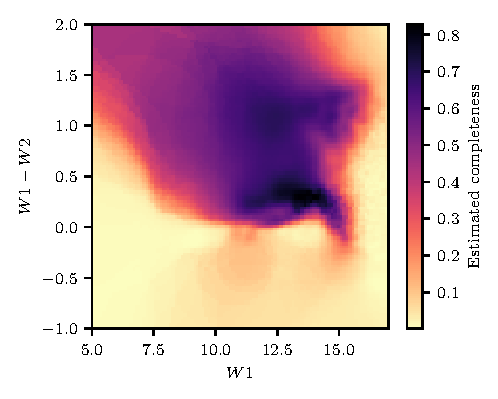
\includegraphics{rlf-images/completeness_wise.pdf}
        \caption{\label{fig:completeness-wise} Estimated completeness as a function of mid-infrared colour and magnitude.}
    \end{figure}

  \section{Giant radio galaxies}
  \label{sec:rlfs-giants}

    \begin{table*}
      \caption[Giant radio galaxies found in RGZ-Ex.]{\label{tab:grg} Giant radio galaxies found in RGZ-Ex. `LLS' is the projected linear size of the source as measured by the maximum angular distance between radio components. The RA/Dec are the coordinates of the host galaxy. s/p indicates spectroscopic/photometric redshift. ${}^L$Existing in literature. ${}^R$Also found by RGZ citizen scientists. ${}^\dagger$Misidentified SDSS host, manually corrected to obtain redshift.}
      \centering
      \begin{footnotesize}\begin{tabular}{c|ccccc}
  \hline\hline
  All\emph{WISE} host (WISEA) & RA (J2000) & Dec (J2000) & $z$ & LLS (Mpc) &\\
  \hline
    J004210.18-080011.3 & 10.54 & -8.00 & $0.65 \pm 0.14$ & 1.6 & p\\ % 3051
    J021008.48+011839.6${}^L$ & 32.54 & 1.31 & $0.86524 \pm 0.0001$ & 1.2 & s\\ % 8420
    J075858.29+355643.6${}^R$ & 119.74 & 35.95 & $0.74748 \pm 0.00013$ & 1.0 & s\\ % 19661
    J080831.68+473523.9${}^R$ & 122.13 & 47.59 & $0.58854 \pm 0.00016$ & 1.1 & s\\ % 21331
    J083034.78+231124.6 & 127.64 & 23.19 & $0.94 \pm 0.13$ & 1.1 & p\\ % 25768
    J090604.03+011114.2 & 136.52 & 1.19 & $0.7975 \pm 0.0004$ & 1.6 & s\\ % 33696
    J093256.81+074212.2 & 143.24 & 7.70 & $1.0032 \pm 0.0003$ & 1.1 & s\\ % 39983
    J093526.80+051729.8${}^R$ & 143.86 & 5.29 & $0.84 \pm 0.04$ & 1.2 & p\\ % 40574
    J094238.72+114337.9 & 145.66 & 11.73 & $0.49 \pm 0.05$ & 1.2 & p\\ % 42294
    J094835.60+535946.4${}^R$ & 147.15 & 54.00 & $0.64 \pm 0.10$ & 1.2 & p\\ % 43609
    J095706.12+292439.2 & 149.28 & 29.41 & $0.71 \pm 0.12$ & 1.5 & p\\ % 45638
    J102335.25+433208.0 & 155.90 & 43.54 & $0.75 \pm 0.09$ & 1.5 & p\\ % 51758
    J102933.99+210345.8${}^R$ & 157.39 & 21.06 & $0.82407 \pm 0.00008$ & 1.1 & s\\ % 53159
    J103043.98+355451.2${}^R$ & 157.68 & 35.91 & $0.64074 \pm 0.00008$ & 1.2 & s\\ % 53433
    J104449.92+234525.6${}^\dagger$ & 161.20 & 23.76 & $0.57712 \pm 0.00009$ & 1.6 & s\\ % 56652
    J110655.98+624759.8${}^R$ & 166.73 & 62.80 & $0.84379 \pm 0.00004$ & 1.1 & s\\ % 61882
    J112900.68+635543.2 & 172.25 & 63.93 & $0.71 \pm 0.06$ & 1.1 & p\\ % 67101
    J112948.20+243922.6 & 172.45 & 24.66 & $0.79 \pm 0.07$ & 1.1 & p\\ % 67288
    J114553.67-003304.7 & 176.47 & -0.55 & $2.0522 \pm 0.0006$ & 1.3 & s\\ % 71048
    J121111.26+534840.4 & 182.80 & 53.81 & $0.74 \pm 0.14$ & 1.1 & p\\ % 77051
    J121152.04+304232.4${}^R$ & 182.97 & 30.71 & $0.47102 \pm 0.00012$ & 1.3 & s\\ % 77229
    J121944.73+174121.3 & 184.94 & 17.69 & $1.5129 \pm 0.0009$ & 1.0 & s\\ % 79128
    J123735.89+544814.4${}^R$ & 189.40 & 54.80 & $1.0271 \pm 0.0006$ & 1.2 & s\\ % 83169
    J123819.16+113444.8 & 189.58 & 11.58 & $0.80 \pm 0.08$ & 1.2 & p\\ % 83310
    J123846.84-032857.5${}^\dagger$ & 189.70 & -3.48 & $0.67 \pm 0.07$ & 1.5 & p\\ % 83402
    J131625.00+272042.8 & 199.10 & 27.35 & $0.69092 \pm 0.00004$ & 1.0 & s\\ % 92344
    J133307.00+045048.6${}^R$ & 203.28 & 4.85 & $1.40534 \pm 0.00016$ & 1.1 & s\\ % 96197
    J141933.36+104706.4${}^R$ & 214.89 & 10.79 & $0.33973 \pm 0.00003$ & 1.0 & s\\ % 107030
    J142008.45+185422.7${}^R$ & 215.04 & 18.91 & $0.63 \pm 0.04$ & 1.4 & p\\ % 107197
    J145057.28+530007.7${}^L$ & 222.74 & 53.00 & $0.91662 \pm 0.00009$ & 1.3 & s\\ % 114664
    J150012.18+604941.3 & 225.05 & 60.83 & $1.6626 \pm 0.0007$ & 1.2 & s\\ % 116901
    J153547.13+432245.0${}^R$ & 233.95 & 43.38 & $0.63891 \pm 0.00007$ & 1.3 & s\\ % 125394
    J154631.18+194819.9 & 236.63 & 19.81 & $0.5917 \pm 0.0002$ & 1.4 & s\\ % 127907
    J160852.10+561110.2${}^R$ & 242.22 & 56.19 & $1.3196 \pm 0.0003$ & 1.3 & s\\ % 132855
    J162200.48+364044.0 & 245.50 & 36.68 & $1.9994 \pm 0.0002$ & 1.1 & s\\ % 135486
    J163004.35+103321.9${}^R$ & 247.52 & 10.56 & $0.85 \pm 0.09$ & 1.2 & p\\ % 136997
    J163125.75+200224.1${}^R$ & 247.86 & 20.04 & $0.62662 \pm 0.00013$ & 1.0 & s\\ % 137251
    J165055.46+394446.6 & 252.73 & 39.75 & $0.58829 \pm 0.00013$ & 1.1 & s\\ % 140491
    J232410.33+045309.6 & 351.04 & 4.89 & $0.76 \pm 0.06$ & 1.4 & p\\ % 156015
    J234440.02-003231.6 & 356.17 & -0.54 & $0.5014 \pm 0.0001$ & 1.0 & s\\ % 157352
      \hline\hline
      \end{tabular}\end{footnotesize}
    \end{table*}

    This appendix describes our search for giant radio galaxies in RGZ-Ex, and the results of this search. It was originally an appendix to \citet{alger21rlfs}. To identify radio sources we assumed that if any two components had the same host galaxy then they were part of the same source. This is a reasonable assumption if all host galaxies are correctly identified, which was not the case. This assumption therefore introduced spurious sources due to galaxies incorrectly identified as host galaxies: not all sources used in \autoref{cha:rlfs} are real sources, and in particular sources of large angular size are likely to be incorrect. Nevertheless RGZ-Ex provides a useful catalogue of \emph{candidate} radio sources, and visual follow-up can confirm whether sources of interest are real.

    H.A. and M.J.A. examined all 296 candidate sources in the RGZ-Ex catalogue with an estimated physical extent larger than 1~Mpc. Of these, 40 were real giant radio galaxies, which we show in \autoref{tab:grg}. We defined `giant radio galaxy' as a radio galaxy with emission extended to physical sizes $\geq 1.0$~Mpc. Other thresholds, such as $0.7$~Mpc, also exist in literature. The physical extents of the remaining 256 candidate sources were overestimated
mostly due to sidelobes/artefacts (103), incorrect source grouping (82), or incorrect SDSS matches (21). The citizen scientists who identified giants are: WizardHowl, DolorousEdd, antikodon, csunjoto, sisifolibre, JeanTate, JKD, PADV, and firejuggler. H.A., together with his summer students, had previously identified 29 of these giants.

    Note that this is a particularly challenging set: sources that are misidentified will often have unusually large estimated extents due to the inclusion of spurious components. The error rate in this set therefore does not reflect the rest of the catalogue.

\section{Visual verification results}
\label{sec:rlfs-verification-appendix}
  
  In \autoref{sec:rlfs-manual-validation} we described our visual verification of the BXID method from \autoref{cha:rlfs}. We list the radio components in the verification set in \autoref{tab:verification-set}. Each row of the table contains the FIRST component, its All\emph{WISE} host galaxy according to BXID, and whether the association is correct according to our visual verification. If an author was particularly unsure about an object, they were able to skip this object, and so are not accounted for in the verification for that object. Verification was weighted by the \citet{dawid79em} maximum likelihood model. This appendix was originally part of \citep{alger21rlfs}.

  \begin{table}
    \caption[Validation objects.]{\label{tab:verification-set} Validation objects. `Agree' is whether or not the authors of \citet{alger21rlfs} agreed with BXID associating the given FIRST object with the given All\emph{WISE} object.}
        \scriptsize\centering
      \begin{tabular}{ccc}
        \hline\hline
        FIRST & All\emph{WISE} & Agree\\\hline
        J000234.9-001421 & J000242.35-001320.5 & n\\
        J002841.1+141654 & J002840.37+141652.7 & y\\
        J003731.4+000156 & J003731.26+000146.7 & y\\
        J005407.5-011158 & J005407.61-011158.9 & y\\
        J011210.3+002203 & J011210.41+002201.9 & y\\
        J012342.4+015849 & J012342.24+015850.4 & y\\
        J013015.1+110653 & J013015.16+110653.4 & y\\
        J013107.7+070343 & J013102.02+070332.0 & y\\
        J014247.9-000039 & J014247.81-000040.3 & y\\
        J014250.0-000032 & J014247.81-000040.3 & n\\
        J020222.3+030138 & J020223.20+030150.4 & y\\
        J020333.8+000853 & J020336.94+000759.3 & y\\
        J021840.1-032311 & J021840.13-032306.0 & y\\
        J023022.0+010834 & J023022.11+010840.0 & y\\
        J024245.3-022535 & J024245.35-022534.6 & y\\
        J025901.0+005350 & J025901.50+005346.1 & y\\
        J033204.1-004757 & J033204.15-004757.1 & y\\
        J073033.2+390413 & J073033.21+390412.9 & y\\
        J073954.1+481810 & J073954.87+481759.5 & y\\
        J074504.9+331247 & J074504.81+331256.2 & y\\
        J074640.4+421709 & J074640.45+421709.1 & y\\
        J074707.9+171719 & J074708.35+171726.5 & y\\
        J075043.6+274838 & J075043.35+274844.8 & n\\
        J075050.3+331937 & J075051.25+331905.0 & y\\
        J075422.2+311253 & J075422.35+311252.5 & y\\
        J075637.0+212006 & J075636.65+212001.4 & y\\
        J082326.1+141438 & J082326.34+141435.9 & y\\
        J082422.5+351121 & J082422.65+351114.6 & y\\
        J082925.9+462618 & J082926.02+462618.5 & y\\
        J083512.4+175441 & J083512.45+175441.1 & y\\
        J084133.5+402035 & J084133.40+402042.8 & y\\
        J084238.4+405305 & J084238.38+405306.6 & n\\
        J084417.3+315845 & J084417.92+315845.9 & y\\
        J084728.5+360700 & J084728.24+360714.6 & y\\
        J084905.5+111448 & J084905.51+111447.8 & y\\
        J085236.8+262006 & J085236.11+262013.4 & y\\
        J085415.6+524930 & J085415.62+524936.7 & y\\
        J090623.2+300746 & J090622.87+300743.9 & y\\
        J091745.1+275049 & J091745.89+275103.8 & y\\
        J091752.0+431614 & J091752.14+431612.7 & y\\
        J092014.4+302907 & J092013.95+302859.3 & y\\
        J092140.5+540118 & J092140.24+540121.1 & y\\
        J092213.0+542157 & J092213.03+542157.2 & y\\
        J092406.9+562703 & J092406.47+562656.2 & y\\
        J092713.1+105841 & J092713.14+105839.8 & y\\
        J093108.6+613447 & J093108.63+613447.2 & y\\
        J093239.6+052308 & J093237.71+052240.7 & n\\
        J093627.8+103610 & J093627.87+103609.7 & y\\
        J093645.2+561435 & J093645.89+561434.2 & y\\
        J094006.8+482651 & J094006.92+482649.2 & y\\\hline\hline
  \end{tabular}
  \begin{tabular}{ccc}
        \hline\hline
        FIRST & All\emph{WISE} & Agree\\\hline
        J094009.5+600403 & J094011.55+600357.6 & n\\
        J094023.7+135123 & J094023.73+135125.2 & y\\
        J094324.5+435341 & J094324.61+435342.0 & y\\
        J094650.8+382015 & J094650.44+382010.9 & y\\
        J095011.8+455319 & J095011.82+455320.0 & y\\
        J095113.5+180211 & J095113.82+180204.2 & n\\
        J095242.4+222638 & J095242.45+222638.0 & y\\
        J095538.7+013546 & J095539.20+013546.1 & y\\
        J095609.9+363441 & J095609.30+363445.4 & y\\
        J095811.8+225056 & J095811.90+225055.5 & y\\
        J100019.2+263516 & J100018.84+263527.5 & y\\
        J101315.9+064520 & J101316.51+064519.0 & y\\
        J101455.2-004716 & J101455.30-004718.3 & y\\
        J102153.5+260429 & J102153.52+260429.6 & y\\
        J102354.7+390653 & J102354.88+390654.0 & y\\
        J102620.4+303600 & J102620.46+303550.4 & y\\
        J102710.4+460254 & J102714.81+460256.4 & n\\
        J102955.9+424906 & J102955.96+424906.7 & y\\
        J103503.9+102404 & J103503.92+102403.6 & y\\
        J103839.9+331200 & J103839.94+331201.1 & y\\
        J104030.5+211624 & J104031.09+211620.6 & n\\
        J104533.8+430025 & J104535.22+430020.8 & y\\
        J104907.5+322903 & J104907.91+322906.6 & y\\
        J105146.9+552257 & J105147.40+552308.4 & y\\
        J105257.5+105418 & J105257.53+105421.5 & y\\
        J105521.6+372641 & J105521.24+372652.4 & y\\
        J105758.8+321605 & J105758.84+321605.3 & y\\
        J110104.9+151618 & J110104.90+151618.2 & y\\
        J110353.2+352320 & J110353.37+352319.9 & y\\
        J110414.4+481345 & J110423.08+481311.0 & n\\
        J111057.7+220756 & J111057.18+220758.3 & y\\
        J111208.5+275207 & J111201.79+275053.8 & n\\
        J111225.2+233159 & J111225.30+233157.9 & y\\
        J111726.3+375336 & J111726.35+375337.0 & y\\
        J111746.1+261151 & J111746.18+261150.9 & y\\
        J111854.3+424708 & J111854.45+424652.8 & y\\
        J112124.4+640417 & J112125.02+640408.6 & y\\
        J112135.3+352330 & J112135.44+352324.9 & y\\
        J112550.9+200631 & J112558.75+200554.3 & y\\
        J112859.7+260923 & J112859.86+260911.3 & y\\
        J113201.1+442639 & J113201.23+442639.4 & y\\
        J113302.5+355408 & J113301.80+355415.3 & y\\
        J113712.7+263301 & J113711.86+263335.1 & y\\
        J113756.3+471314 & J113756.31+471314.1 & y\\
        J113906.6+230602 & J113906.68+230602.1 & y\\
        J114325.0+600721 & J114323.90+600737.1 & y\\
        J114759.7+370305 & J114759.22+370311.2 & y\\
        J114916.7+083022 & J114916.33+083040.5 & n\\
        J115010.9+063340 & J115010.93+063340.5 & y\\
        J115308.6+374851 & J115316.96+374850.0 & y\\\hline\hline
  \end{tabular}
\end{table}
\begin{table}
    \scriptsize\centering
  \begin{tabular}{ccc}
        \hline\hline
        FIRST & All\emph{WISE} & Agree\\\hline
        J115448.7+472222 & J115448.67+472223.7 & y\\
        J115603.7+584704 & J115603.48+584706.1 & y\\
        J115605.9+343230 & J115605.64+343229.4 & y\\
        J115653.0+572338 & J115645.38+572151.7 & y\\
        J120138.0+230922 & J120137.97+230922.2 & y\\
        J120752.8+533808 & J120752.85+533807.3 & y\\
        J120943.3-021934 & J120942.89-021943.0 & y\\
        J121045.6+190225 & J121045.68+190227.0 & y\\
        J121207.6+115412 & J121207.72+115413.8 & y\\
        J121211.3+485951 & J121211.86+485952.0 & y\\
        J121406.7+002634 & J121406.73+002635.0 & y\\
        J122518.0+350258 & J122517.85+350301.9 & y\\
        J122525.1+451530 & J122524.71+451508.5 & y\\
        J122640.9+430508 & J122640.82+430509.2 & y\\
        J123429.8+260107 & J123434.79+260134.3 & n\\
        J123633.1+100928 & J123633.12+100928.7 & y\\
        J124839.3+411522 & J124839.42+411522.3 & n\\
        J125129.2+551012 & J125128.76+551009.3 & y\\
        J130005.8+524801 & J130006.14+524803.0 & y\\
        J130132.1+511351 & J130132.32+511352.5 & y\\
        J131104.4+464936 & J131104.45+464934.0 & y\\
        J131452.2+252811 & J131446.81+252820.8 & n\\
        J132033.8+332639 & J132033.59+332639.0 & n\\
        J132257.5+191134 & J132257.53+191133.9 & y\\
        J132529.3+230734 & J132529.35+230733.8 & y\\
        J132546.8+052453 & J132546.86+052454.1 & y\\
        J132637.7+112110 & J132637.92+112108.8 & y\\
        J132831.8+104339 & J132831.88+104338.8 & y\\
        J132932.3+131839 & J132932.32+131839.6 & y\\
        J133022.8+311904 & J133022.83+311902.8 & y\\
        J133453.3+405653 & J133454.13+405650.6 & y\\
        J133741.1+124302 & J133741.13+124303.1 & y\\
        J133823.6+103337 & J133823.67+103341.9 & y\\
        J134651.2+415154 & J134651.06+415156.1 & y\\
        J134704.3+110622 & J134704.35+110622.7 & y\\
        J134752.7+555046 & J134752.71+555048.6 & y\\
        J134831.7+164325 & J134831.57+164328.2 & y\\
        J134949.8+385539 & J134949.93+385542.8 & y\\
        J135106.5+074534 & J135106.50+074534.2 & y\\
        J135107.7+615502 & J135107.75+615502.1 & y\\
        J135658.5+134028 & J135659.15+134017.0 & y\\
        J135833.9+180021 & J135834.03+180020.4 & y\\
        J140630.7+554017 & J140629.32+554009.9 & y\\
        J140804.2+503019 & J140804.10+503021.1 & y\\
        J141226.7+454125 & J141226.54+454125.5 & y\\
        J141245.0+495213 & J141243.84+495206.4 & y\\
        J141317.4+325306 & J141317.50+325306.8 & y\\
        J141723.8+543639 & J141724.33+543629.5 & y\\
        J141938.8+312146 & J141940.16+312138.8 & y\\
        J142515.3+175526 & J142513.89+175525.7 & y\\\hline\hline
  \end{tabular}
  \begin{tabular}{ccc}
        \hline\hline
        FIRST & All\emph{WISE} & Agree\\\hline
        J142829.5+070836 & J142829.60+070836.3 & y\\
        J143411.0+170036 & J143411.18+170035.7 & y\\
        J143624.0-001057 & J143623.89-001100.8 & y\\
        J143742.6+104412 & J143742.69+104412.8 & y\\
        J143840.8+475355 & J143841.08+475356.1 & y\\
        J143909.1+430847 & J143909.08+430847.8 & y\\
        J144135.8+102246 & J144135.91+102245.1 & y\\
        J144333.6+275229 & J144333.02+275250.2 & y\\
        J145012.3+471739 & J145012.33+471738.7 & y\\
        J145103.7+452459 & J145102.66+452520.5 & n\\
        J145401.6+141009 & J145401.70+141009.6 & y\\
        J150158.7+191413 & J150158.87+191405.3 & y\\
        J150743.9+352720 & J150743.62+352724.1 & y\\
        J151141.6-003209 & J151142.01-003213.0 & y\\
        J151315.5+403107 & J151315.56+403107.7 & y\\
        J151518.7+230256 & J151518.67+230257.3 & y\\
        J151703.6+105947 & J151703.68+105947.6 & y\\
        J151736.8+610856 & J151736.83+610857.7 & y\\
        J152121.6+281635 & J152120.68+281626.2 & y\\
        J152714.8+310425 & J152714.88+310424.7 & y\\
        J153428.9+272134 & J153429.68+272120.8 & y\\
        J154245.3+100919 & J154245.71+100917.8 & y\\
        J154901.6+103159 & J154901.40+103152.6 & y\\
        J154925.2+395316 & J154926.17+395303.7 & y\\
        J155206.3-005348 & J155206.58-005339.3 & y\\
        J155457.3+344637 & J155458.45+344644.7 & y\\
        J155743.5+272752 & J155743.52+272752.8 & y\\
        J160130.0+083848 & J160130.07+083850.7 & y\\
        J160534.8+441220 & J160535.55+441221.5 & y\\
        J160859.2+400135 & J160901.32+400230.7 & n\\
        J161545.4+231617 & J161545.14+231617.2 & y\\
        J161930.4+085533 & J161930.51+085532.6 & y\\
        J162228.0+264743 & J162228.70+264736.7 & y\\
        J162750.4+473624 & J162750.55+473623.5 & y\\
        J162904.2+470852 & J162904.34+470853.0 & y\\
        J163038.7+214740 & J163037.43+214748.9 & n\\
        J163323.6+424051 & J163323.61+424051.9 & y\\
        J163327.5+242426 & J163327.87+242427.4 & y\\
        J163533.8+454557 & J163534.00+454554.3 & y\\
        J164211.2+512029 & J164211.27+512029.3 & y\\
        J165549.1+375923 & J165549.01+375923.6 & y\\
        J165620.0+363402 & J165619.89+363403.9 & y\\
        J165700.5+474820 & J165659.58+474809.0 & y\\
        J171406.2+292712 & J171404.16+292704.0 & n\\
        J172126.4+374446 & J172126.46+374446.6 & y\\
        J222627.7-005010 & J222627.77-005010.8 & y\\
        J223636.4-013827 & J223636.48-013827.2 & y\\
        J225619.0+143257 & J225621.96+143351.4 & y\\
        J232410.1+001315 & J232410.15+001314.5 & y\\
        J234727.9-000919 & J234727.65-000912.9 & y\\\hline\hline
  \end{tabular}
\end{table}

\section{2-Wasserstein begets Faraday moments}
  \label{sec:faraday-w2-to-faraday-moments}
    Minimising the 2-Wasserstein distance between a model FDF and the simple manifold gives the second Faraday moment of that FDF. This appendix demonstrates that fact, and was originally part of \citet{alger2021interpretable}. Let $\tilde F$ be the sum-normalised model FDF and let $\tilde S$ be the sum-normalised simple model FDF:
    \begin{align}
      \tilde F(\phi) &= \frac{A_0 \delta(\phi - \phi_0) + A_1 \delta(\phi - \phi_1)}{A_0 + A_1}\\
      \tilde S(\phi; \phi_w) &= \delta(\phi - \phi_w).
    \end{align}
    The $W_2$ distance, usually defined on probability distributions, can be extended to one-dimensional complex functions $A$ and $B$ by normalising them:
      \begin{align}
        \label{eq:faraday-w2}
        D_{W_2}\infdivx{A}{B}^2 &= \inf_{\gamma \in \Gamma(A, B)} \iint_{\phi_{\min}}^{\phi_{\max}} |x - y|^2\ \mathrm{d}\gamma(x, y) \\
        \label{eq:faraday-normalised}
        \tilde A(\phi) &= \frac{|A(\phi)|}{\int_{\phi_{\min}}^{\phi_{\max}} |A(\theta)|\ \mathrm{d}\theta}\\
        \tilde B(\phi) &= \frac{|B(\phi)|}{\int_{\phi_{\min}}^{\phi_{\max}} |B(\theta)|\ \mathrm{d}\theta}
      \end{align}
      where $\Gamma(A, B)$ is the set of couplings of $A$ and $B$, i.e. the set of joint probability distributions that marginalise to $A$ and $B$; and $\inf_{\gamma \in \Gamma(A, B)}$ is the infimum over $\Gamma(A, B)$. This can be interpreted as the minimum cost to `move' one probability distribution to the other, where the cost of moving one unit of probability mass is the squared distance it is moved.

    The set of couplings $\Gamma(\tilde F, \tilde S)$ is the set of all joint probability distributions $\gamma$ such that
    \begin{align}
      \int_{\phi_{\min}}^{\phi_{\max}} \gamma(\phi, \varphi)\ \mathrm{d}\phi &= \tilde S(\varphi; \phi_w),\\
      \int_{\phi_{\min}}^{\phi_{\max}} \gamma(\phi, \varphi)\ \mathrm{d}\varphi &= \tilde F(\phi).
    \end{align}
    The coupling that minimises the integral in \autoref{eq:faraday-w2} will be the optimal transport plan between $\tilde F$ and $\tilde S$. Since $\tilde F$ and $\tilde S$ are defined in terms of delta functions, the optimal transport problem reduces to a discrete optimal transport problem and the optimal transport plan is:
    \begin{equation}
      \gamma(\phi, \varphi) = \frac{A_0 \delta(\phi - \phi_0) + A_1 \delta(\phi - \phi_1)}{A_0 + A_1} \delta(\varphi - \phi_w).
    \end{equation}
    In other words, to move the probability mass of $\tilde S$ to $\tilde F$, a fraction $A_0/(A_0 + A_1)$ is moved from $\phi_w$ to $\phi_0$ and the complementary fraction $A_1/(A_0 + A_1)$ is moved from $\phi_w$ to $\phi_1$. Then:
    \begin{align}
      D_{W_2}\infdivx{\tilde F}{\tilde S}^2 &= \iint_{\phi_{\min}}^{\phi_{\max}} |\phi - \varphi|^2\ \mathrm{d}\gamma(\phi, \varphi)\\
        &= \frac{A_0 (\phi_0 - \phi_w)^2 + A_1 (\phi_1 - \phi_w)^2}{A_0 + A_1}.
    \end{align}
    To obtain the $W_2$ distance to the simple manifold, we need to minimise this over $\phi_w$. Differentiate with respect to $\phi_w$ and set equal to zero to find
    \begin{equation}
      \phi_w = \frac{A_0 \phi_0 + A_1 \phi_1}{A_0 + A_1}.
    \end{equation}
    Substituting this back in, we find
    \begin{align}
      \varsigma_{W_2}(F)^2 &= \frac{A_0 A_1}{A_0 + A_1}(\phi_0 - \phi_1)^2
    \end{align}
    which is the Faraday moment.

\section{Euclidean distance in the no-RMSF case}
\label{sec:faraday-euclidean-calculation}

  In this appendix, originally from \citet{alger2021interpretable}, we calculate the minimised Euclidean distance evaluated on a model FDF (\autoref{eq:faraday-true-fdf}). Let $\tilde F$ be the sum-normalised model FDF and let $\tilde S$ be the normalised simple model FDF:
  \begin{align}
    \tilde F(\phi) &= \frac{A_0 \delta(\phi - \phi_0) + A_1 \delta(\phi - \phi_1)}{A_0 + A_1}\\
    \tilde S(\phi; \phi_e) &= \delta(\phi - \phi_e).
  \end{align}

  The Euclidean distance between $\tilde F$ and $\tilde S$ is then
  \begin{align}
    &D_E\infdivx{\tilde F(\phi)}{\tilde S(\phi; \phi_e)}^2\\
    &= \int_{\phi_{\min}}^{\phi_{\max}} \left|\tilde F(\phi) - \delta(\phi - \phi_e) \right|^2\ \mathrm{d}\phi.
  \end{align}

  Assume $\phi_0 \neq \phi_1$ (otherwise, $D_E$ will always be either $0$ or $2$). If $\phi_e = \phi_0$, then
  \begin{align}
    &D_E\infdivx{\tilde F(\phi)}{\tilde S(\phi; \phi_e)}^2\\
      &= \frac{1}{(A_0 + A_1)^2} \int_{\phi_{\min}}^{\phi_{\max}} A_1^2 \left|\delta(\phi - \phi_1) - \delta(\phi - \phi_0) \right|^2\ \mathrm{d}\phi\\
      &= \frac{2 A_1^2}{(A_0 + A_1)^2}
  \end{align}
  and similarly for $\phi_e = \phi_1$. If $\phi_e \neq \phi_0$ and $\phi_e \neq \phi_1$, then
  \begin{equation}
    D_E\infdivx{\tilde F(\phi)}{\tilde S(\phi; \phi_e)}^2 = \frac{A_0^2 + A_1^2 + 1}{(A_0 + A_1)^2}.
  \end{equation}
  The minimised Euclidean distance when $\phi_0 \neq \phi_1$ is therefore
  \begin{align}
      D_E(F) &= \min_{\phi_e \in \mathbb{R}} D_E\infdivx{F(\phi)}{F_{\mathrm{simple}}(\phi; \phi_e)}\\
          &= \sqrt{2} \frac{\min(A_0, A_1)}{A_0 + A_1}.
  \end{align}
  If $\phi_0 = \phi_1$, then the minimised Euclidean distance is 0.

\section{Hyperparameters for LR and XGB}
\label{sec:faraday-hyperparameters}

  This section contains tables of the hyperparameters that we used for our classifiers in \autoref{cha:faraday} and was originally an appendix to \citet{alger2021interpretable}. \autoref{tab:faraday-hyperparameters-xgb} and \autoref{tab:faraday-hyperparameters-lr} tabulate the hyperparameters for XGB and LR respectively for the `ATCA' dataset. \autoref{tab:faraday-hyperparameters-xgb-askap12} and \autoref{tab:faraday-hyperparameters-lr-askap12} tabulate the hyperparameters for XGB and LR respectively for the `ASKAP' dataset.

  \begin{table}[htbp]
    \caption{\label{tab:faraday-hyperparameters-xgb} XGB hyperparameters for the `ATCA' dataset.}
    \centering
    \begin{tabular}{ll}
      \hline\hline
      Parameter & Value\\\hline
      colsample\textunderscore{}bytree & 0.912\\
      gamma & 0.532\\
      learning\textunderscore{}rate & 0.1\\
      max\textunderscore{}depth & 7\\
      min\textunderscore{}child\textunderscore{}weight & 2\\
      scale\textunderscore{}pos\textunderscore{}weight & 1\\
      subsample & 0.557\\
      n\textunderscore{}estimators & 135\\
      reg\textunderscore{}alpha & 0.968\\
      reg\textunderscore{}lambda & 1.420\\
      \hline\hline
    \end{tabular}
  \end{table}

  \begin{table}[htbp]
    \caption{\label{tab:faraday-hyperparameters-lr} LR hyperparameters for the `ATCA' dataset.}
    \centering
    \begin{tabular}{ll}
      \hline\hline
      Parameter & Value\\\hline
      penalty & L1\\
      C & 1.668\\
      \hline\hline
    \end{tabular}
  \end{table}

  \begin{table}[htbp]
    \caption{\label{tab:faraday-hyperparameters-xgb-askap12} XGB hyperparameters for the `ASKAP' dataset.}
    \centering
    \begin{tabular}{ll}
      \hline\hline
      Parameter & Value\\\hline
      colsample\textunderscore{}bytree & 0.865\\
      gamma & 0.256\\
      learning\textunderscore{}rate & 0.1\\
      max\textunderscore{}depth & 6\\
      min\textunderscore{}child\textunderscore{}weight & 1\\
      scale\textunderscore{}pos\textunderscore{}weight & 1\\
      subsample & 0.819\\
      n\textunderscore{}estimators & 108\\
      reg\textunderscore{}alpha & 0.049\\
      reg\textunderscore{}lambda & 0.454\\
      \hline\hline
    \end{tabular}
  \end{table}

  \begin{table}[htbp]
    \caption{\label{tab:faraday-hyperparameters-lr-askap12} LR hyperparameters for the `ASKAP' dataset.}
    \centering
    \begin{tabular}{ll}
      \hline\hline
      Parameter & Value\\\hline
      penalty & L2\\
      C & 0.464\\
      \hline\hline
    \end{tabular}
  \end{table}

\section{Predictions on real data}
\label{sec:faraday-real-data-fig}

  This appendix, originally part of \citet{alger2021interpretable}, contains \autoref{fig:faraday-all-observed-fdfs-lr} and \autoref{fig:faraday-all-observed-fdfs-xgb}. These show the predicted probability of being Faraday complex for all real data used in \autoref{cha:faraday}, drawn from \citet{livingston21faraday} and \citet{osullivan_broad-band_2017}.

  \begin{figure*}
    \centering
    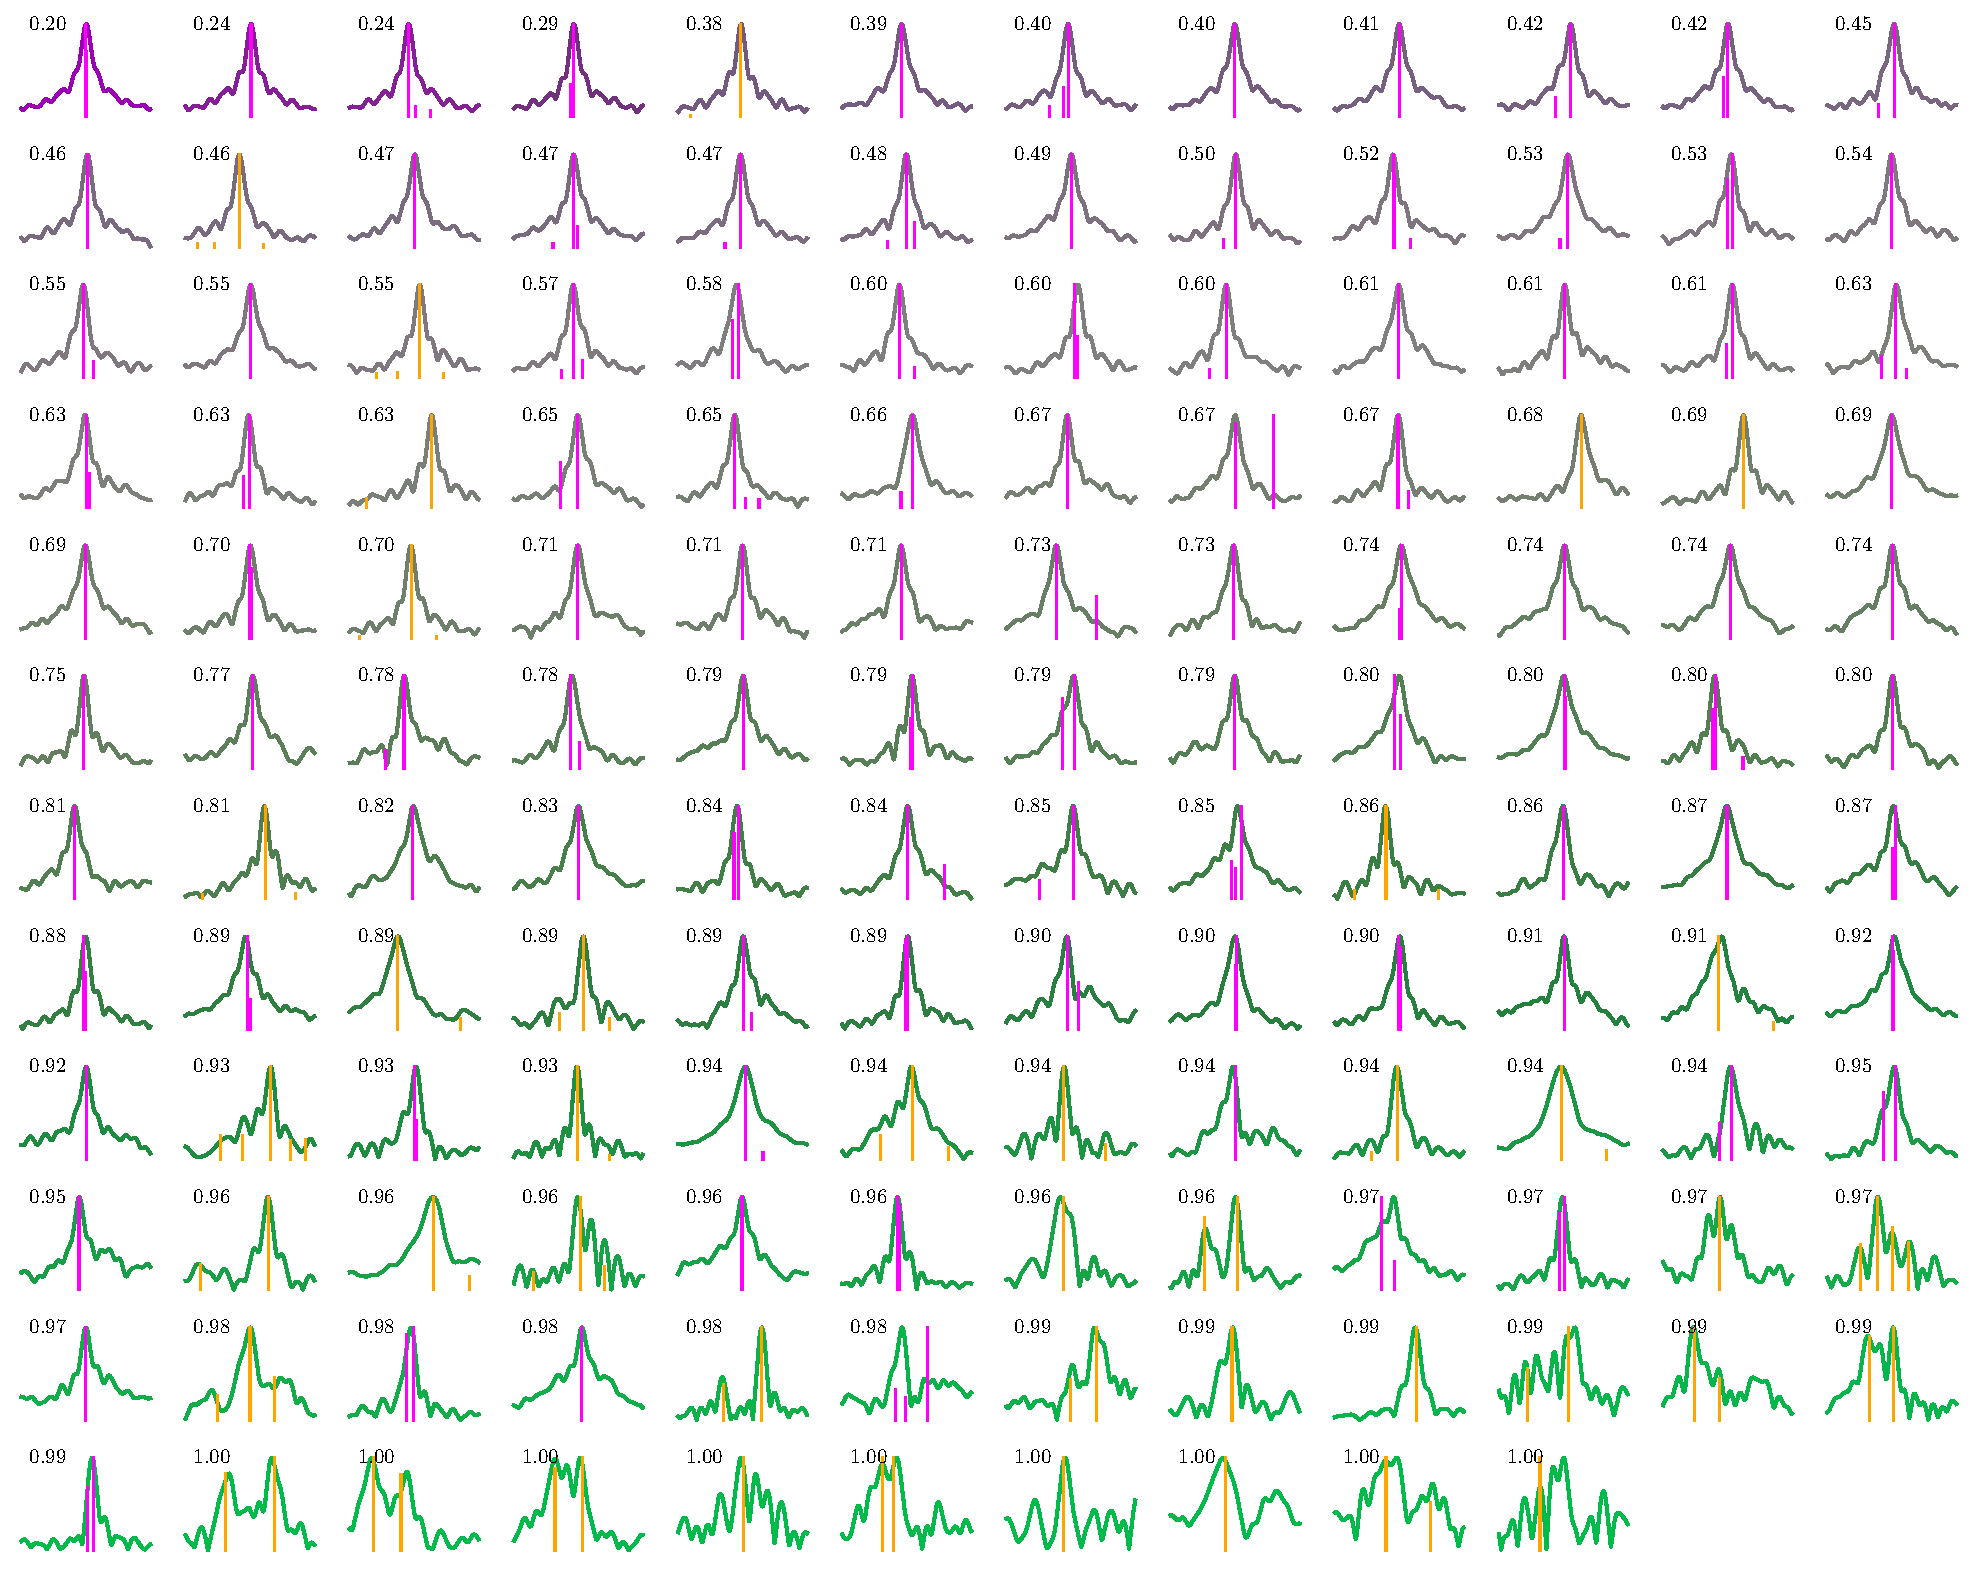
\includegraphics[width=\linewidth]{faraday-images/both_spectra_lr.pdf}
    \caption[The 142 observed FDFs ordered by LR-estimated probability of being Faraday complex.]{The 142 observed FDFs ordered by LR-estimated probability of being Faraday complex. Livingston-identified components are shown in orange while O'Sullivan-identified components are shown in magenta. Simpler FDFs (as deemed by the classifier) are shown in purple while more complex FDFs are shown in green, and the numbers overlaid indicate the LR estimate. A lower number indicates a lower probability that the corresponding source is complex, i.e. lower numbers correspond to simpler spectra.}
    \label{fig:faraday-all-observed-fdfs-lr}
  \end{figure*}

  \begin{figure*}
    \centering
    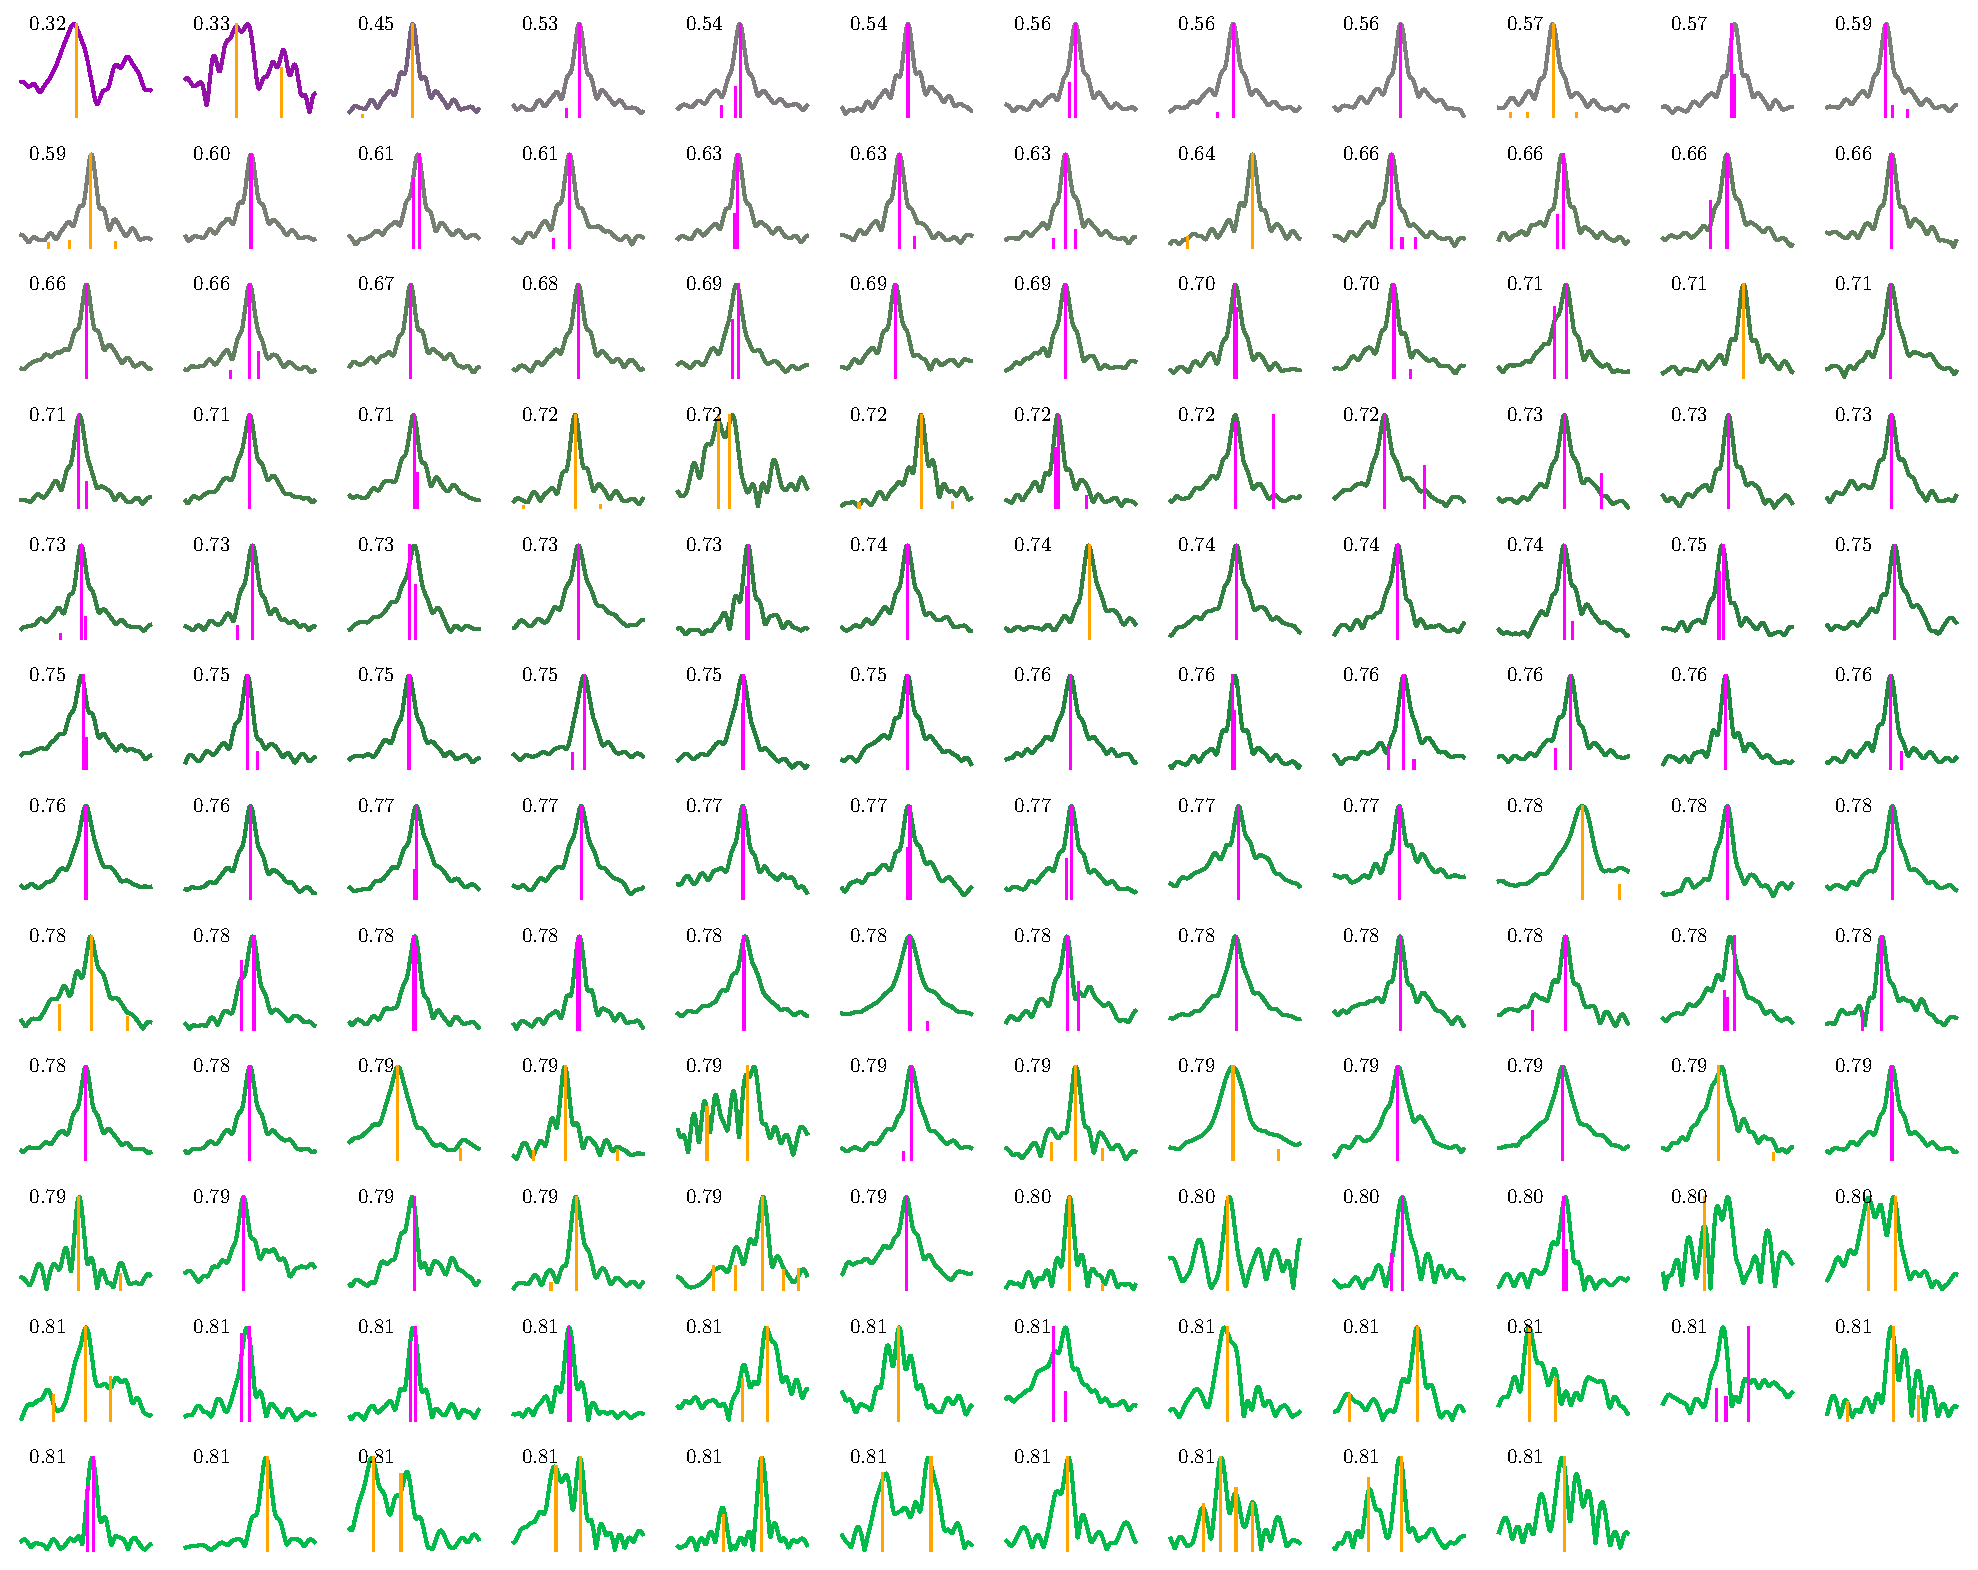
\includegraphics[width=\linewidth]{faraday-images/both_spectra_xgb.pdf}
    \caption[The 142 observed FDFs ordered by XGB-estimated probability of being Faraday complex.]{The 142 observed FDFs ordered by XGB-estimated probability of being Faraday complex. Livingston-identified components are shown in orange while O'Sullivan-identified components are shown in magenta. Simpler FDFs (as deemed by the classifier) are shown in purple while more complex FDFs are shown in green, and the numbers overlaid indicate the XGB estimate. A lower number indicates a lower probability that the corresponding source is complex, i.e. lower numbers correspond to simpler spectra.}
    \label{fig:faraday-all-observed-fdfs-xgb}
  \end{figure*}

\section{Simulating observed FDFs}
\label{sec:faraday-simulating}

  This appendix was originally part of \citet{alger2021interpretable} and describes how we simulated FDFs in \autoref{cha:faraday}. We simulated FDFs by approximating them by arrays of complex numbers. An FDF $F$ is approximated on the domain $[-\phi_{\max}, \phi_{\max}]$ by a vector $\vec F \in \mathbb R^d$:
    \begin{equation}
      \label{eq:faraday-vec-f}
      \vec F_j = \sum_{k = 0}^1 A_k \delta(-\phi_{\max} + j \delta \phi - \phi_k)
    \end{equation}
    where $\delta\phi = (\phi_{\max} - \phi_{\min}) / d$ and $d$ is the number of Faraday depth samples in the FDF.
    $\vec F$ is sampled by uniformly sampling its parameters:
    \begin{align}
      \label{eq:faraday-model-distributions}
      \phi_k &\in [\phi_{\min}, \phi_{\min} + \delta\phi, \dots, \phi_{\max}]\\
      A_k &\sim \mathcal U(0, 1).
    \end{align}
    We then generate a vector polarisation spectrum $\vec P \in \mathbb R^m$ from $\vec F$ using a \autoref{eq:faraday-discrete-f-to-p}:
    \begin{equation}
      \label{eq:faraday-discrete-f-to-p}
      \vec P_\ell = \sum_{j = 0}^{j} F_j e^{2i(\phi_{\min} + j\delta_\phi)\lambda^2_\ell}\ \mathrm{d}\phi.
    \end{equation}
    $\lambda^2_\ell$ is the discretised value of $\lambda^2$ at the $\ell$th index of $\vec P$. This requires a set of $\lambda^2$ values, which depends on the dataset being simulated. These values can be treated as the channel wavelengths at which the polarisation spectrum was observed. We then add Gaussian noise with variance $\sigma^2$ to each element of $\vec P$ to obtain a discretised noisy observation $\hat{\vec{P}}$. Finally, we perform RM synthesis using the Canadian Initiative for Radio Astronomy Data Analysis \texttt{RM} package\footnote{\url{https://github.com/CIRADA-Tools/RM}}, which is a \texttt{Python} module that implements a discrete version of RM synthesis:
    \begin{equation}
      \label{eq:faraday-discrete-rm-synthesis}
      \hat{\vec{F}}_j = m^{-1} \sum_{\ell = 1}^m \vec{\hat P}_\ell e^{-2i(\phi_{\min} + j\delta_\phi)\lambda^2_\ell}.
    \end{equation}